\section{Module de croissance du zooplancton à deux proies}

\subsection{Description du module}

\par{
Dans le quatrième cours on a agrandis le modèle mathématique. On considére maintenant deux espèce de
proies qui sont consommées par le mésozooplancton de façon sélectif ou non-sélectif. Du coup le modèle
conceptuel se changera. On peut admirer le nouveau modèle conceptuel dans la figure~\ref{fig:partie2DiagConc}.
}

\begin{figure}[h!]
  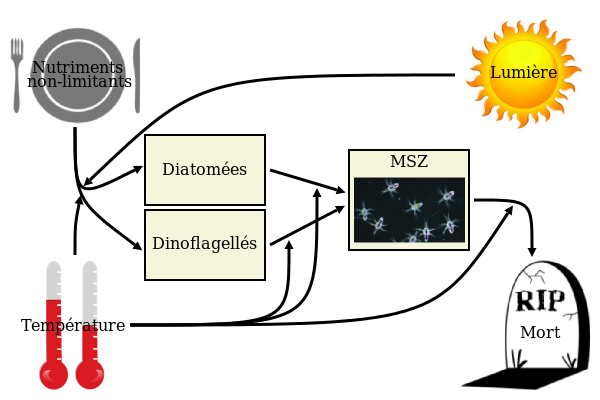
\includegraphics[width=\textwidth]{partie2/diagConc.png}
  \caption{Le modèle conceptuel du système étudié dans le cinquième cours. Par rapport
au modèle conceptuel du quatrième cours (voir figure~\ref{fig:partie1DiagConcept}) on
a augmonter les nombres des espèces (des diatomées et des dinoflagellés) qui peuvent
servir comme proie.
}
  \label{fig:partie2DiagConc}
\end{figure}

\par{
Puisque le diagramme conceptuel était changé on doit revaloriser les équations. Les équations nouveux regardent
comme suit:
}

\begin{equation}
  {{d[DA]}\over{dt}} =
  \mu_{DA} [DA] - graz_{MSZ/DA} [MSZ]
  \label{eq:partie2DiffEq1}
\end{equation}
\begin{equation}
  {{d[DINO]}\over{dt}} =
  \mu_{DINO} [DINO] - graz_{MSZ/DINO} [MSZ]
  \label{eq:partie2DiffEq2}
\end{equation}
\begin{equation}
  {{d[MSZ]}\over{dt}} =
  \left (
    (1- eges_{MSZ}) graz_{MSZ} Y_{MSZ} - mm_{MSZ}
  \right ) [MSZ]
  \label{eq:partie2DiffEq3}
\end{equation}


\begin{equation}
  graz_{MSZ} = graz_{MSZ/DA} + graz_{MSZ/DINO}
  \label{eq:partie2grazMsz}
\end{equation}

\par{
Dans le cas du grazing non sélectif, on considére aussi les équations suivants:
}

\begin{equation}
  [PHYTO] = [DA] + [DINO]
  \label{eq:partie2nonSelEq1}
\end{equation}
\begin{equation}
  graz_{MSZ} = g_{MSZ} max(T) {{[PHYTO]^2}\over{kg_{MSZ}^2 + [PHYTO]^2}}
  \label{eq:partie2nonSelEq2}  
\end{equation}
\begin{equation}
  graz_{MSZ/DA} = graz_{MSZ} {{[DA]}\over{[PHYTO]}}
  \label{eq:partie2nonSelEq2}
\end{equation}
\begin{equation}
  graz_{MSZ/DINO} = graz_{MSZ} {{[DINO]}\over{[PHYTO]}}
  \label{eq:partie2nonSelEq3}
\end{equation}

\par{
Et dans le cas du grazing sélectif, on considére plutôt les équations suivis:
}

\begin{equation}
  graz_{MSZ/DA} = g_{MSZ} max(T) {{\left ( {{[DA]}\over{kg_{MSZ/DA}}}\right )^2}\over
{1 + \left ( {{[DA]}\over{kg_{MSZ/DA}}} \right )^2 + \left ( {{[DINO]}\over{kg_{MSZ/DINO}}} \right )^2}}
  \label{eq:partie2selEq1}
\end{equation}
\begin{equation}
  graz_{MSZ/DINO} = g_{MSZ} max(T) {{\left ( {{[DINO]}\over{kg_{MSZ/DINO}}}\right )^2}\over
{1 + \left ( {{[DA]}\over{kg_{MSZ/DA}}} \right )^2 + \left ( {{[DINO]}\over{kg_{MSZ/DINO}}} \right )^2}}
  \label{eq:partie2selEq2}
\end{equation}
\begin{equation}
  graz_{MSZ} = g_{MSZ/DA} + g_{MSZ/DINO}
  \label{eq:partie2selEq3}
\end{equation}

\par{
Par rapport au travail pratique précendent on peut garder tous les valeurs pour les différents paramètres.
Seulement pour le cas du grazing sélectif, on introduire deux constantes de grazing différentes pour les
deux espèces. Ces constantes ont les valeurs suivantes:
}
\[
kg_{MSZ/DA} = 10 {^{mmol~C}/_{m^3}}
\]
\[
kg_{MSZ/DINO} = 20 {^{mmol~C}/_{m^3}}
\]

\par{

}

\begin{table}[h!]
\begin{center}
\begin{tabular}{ | c | c | c | c | c | c | }
\hline
Variable & Reference & Test 1 & Test 2 & Test 3 & Test 4 \\
\hline
DA & $20$ & $30$ & $10$ & $20$ & $20$ \\
DINO & $20$ & $10$ & $30$ & $20$ & $20$ \\
MSZ & $10$ & $10$ & $10$ & $1$ & $20$ \\
\hline
\end{tabular}
\end{center}
  \caption{Les conditions initiales pour en DA, DINO et MSZ pour les tests different.}
  \label{tab:partie2params}
\end{table}

\subsection{Simulation de référence}

\begin{figure}
  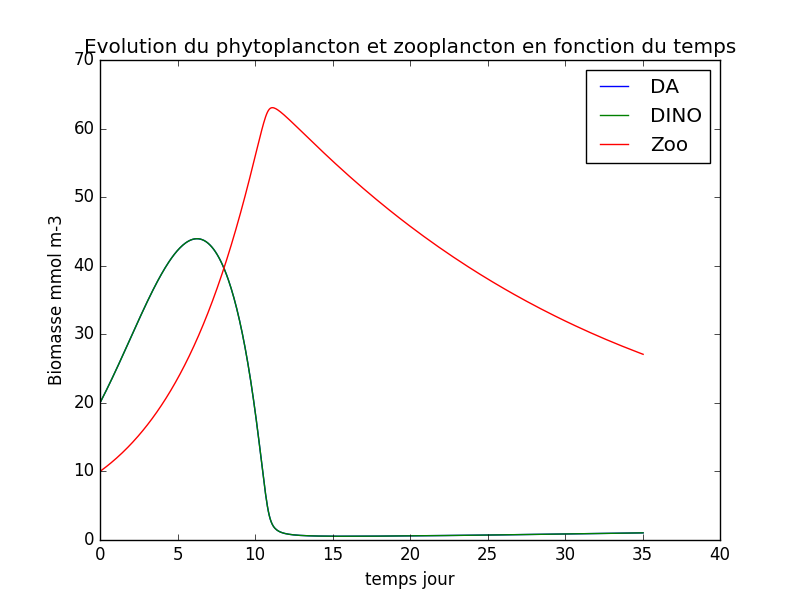
\includegraphics[width=.5\textwidth]{partie2/1Nonselec.png}\hfill
  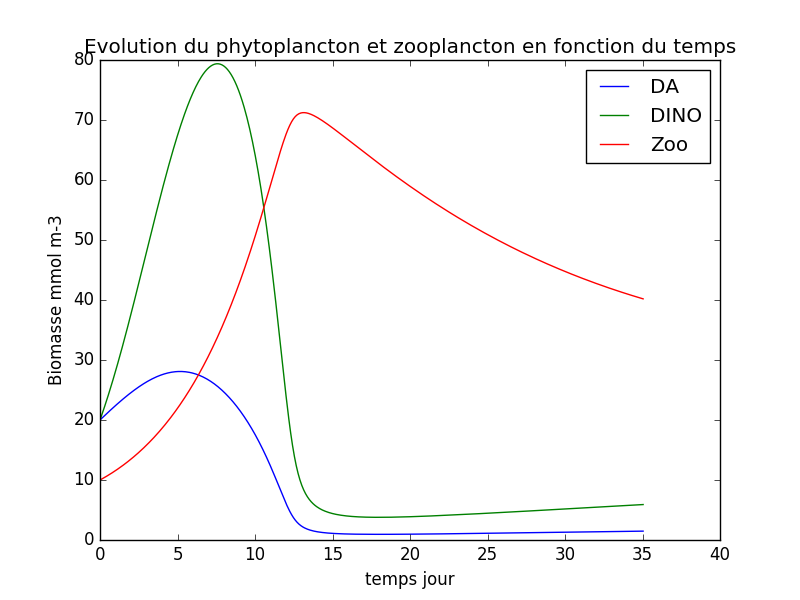
\includegraphics[width=.5\textwidth]{partie2/1Selec.png}
  \caption{Comparison 
Le graphe à droite montre \todo}
  \label{fig:partie2Ref}
\end{figure}

Dans le cas d'un grazing non s\'electif, les deux espèces phytoplanctoniques croissent de la même manière, ce qui fait que les courbes d'évolution de la biomasse sont confondues. En effet, pour les deux espèces, tous les paramètres sont égaux, ainsi que les concentrations initiales. Le maximum de biomasse phytoplanctonique est atteint après 7 jours et a une valeur de 45 mmol.m-3, tandis que le maximum de la biomasse zooplanctonique est atteint après 13 jours et a une valeur de 65 mmol.m-3. Contrairement au TP précédent, la valeur maximum du zooplancton parait supérieure à celle du phytoplancton. Cependant, il faut tenir compte du fait que deux populations de phytoplancton sont présentes, et donc que la concentration maximum de phytoplancton est en fait plus importante que celle du zooplancton.\\
Dans le cas d'un grazing s\'electif, Les deux populations de phytoplancton n'ont ici plus la même évolution. La concentration maximum des Dinoglagellés est atteinte après 7 jours (comme dans le cas non sélectif) mais a une valeur de 80 mmol.m-3, tandis que celle des Diatomées est atteinte après 5 jours, et a une valeur de 30 mmol.m-3. De plus, la concentration maximum du zooplancton est atteinte après 15 jours et a une valeur de 70 mmol.m-3.\\
En effet, les constantes de demi saturation du taux de grazing des deux espèces de phytoplancton sont ici différentes. Une des espèce a le même que dans le cas du non sélectif (les Diatomées), mais l'affinité pour les Dinoflagellés est plus faible. Ceci fait que les Dinoflagellés ont donc la possibilité d'atteindre une concentration maximum plus importante, et que les Diatomées ont une concentration maximum plus faible. 
De plus, on peut voir que la décroissance des Dinoflagellés est beaucoup plus rapide que celle des Diatomées. En effet, au jour 6, la concentration en Dinoflagellés est très importante et celle en Diatomées est faible. Or, on peut voir dans l'équation du taux de grazing (Equation \ref{eq:partie2selEq2}) du Dinoflagellé que si la concentration en Dinoflagellés est grande et que la concentration en Diatomées est faible, alors le taux de grazing des Dinoflagellés est grand. Ceci explique la décroissance rapide des Dinoflagellés. A l'inverse, si on regarde l'équation du taux de grazing des Diatomées (Equation), si la concentration en Dinoflagellés est grande et que la concentration en Diatomées est faible, alors plus le taux de grazing des Diatomées est faible. Ainsi, la population de Diatomée a une décroissance beaucoup plus lente.\\
De plus, on voit que les concentrations minimales ne sont pas les mêmes. En effet, le zooplancton a la capacité d'utiliser plus efficacement les Diatomées à faible concentration que les Dinoflagellés, c'est pourquoi la concentration minimum en Diatomée est plus faible.


\subsection{Tests de la sensitivité}

\begin{figure}
  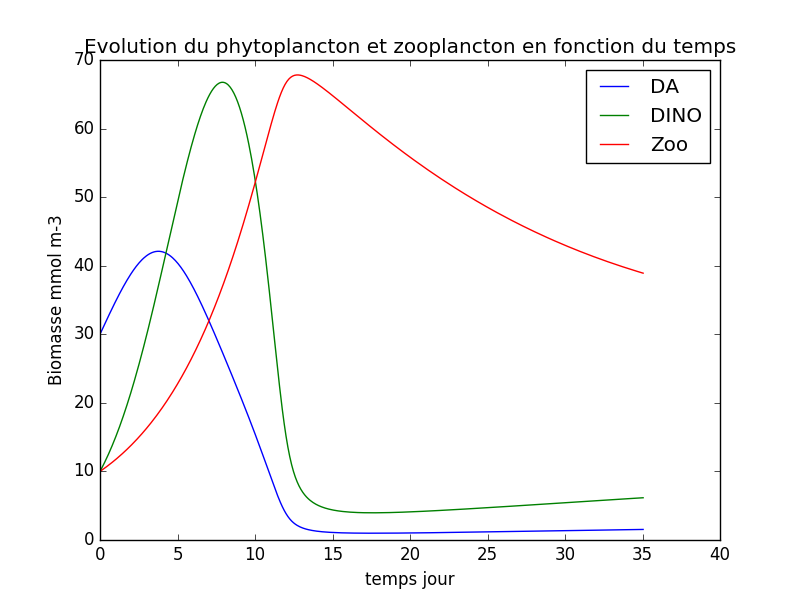
\includegraphics[width=.5\textwidth]{partie2/test1sel.png}\hfill
  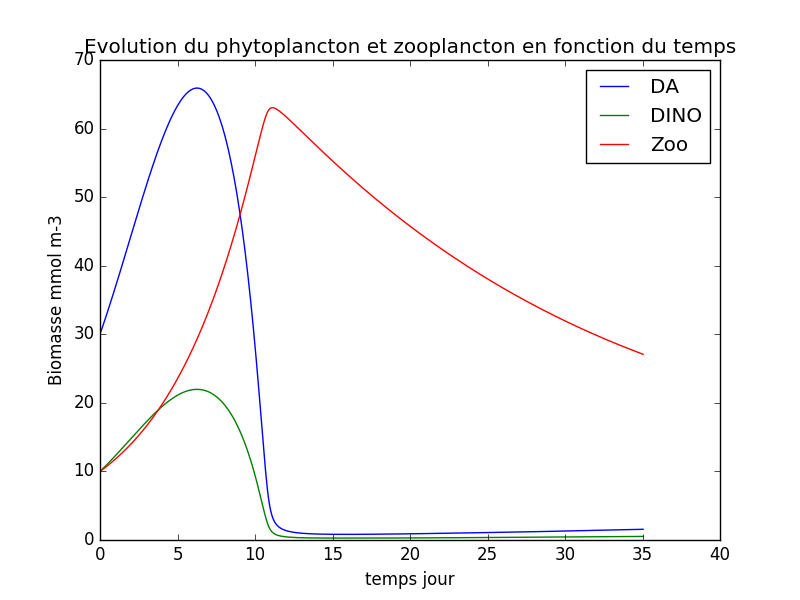
\includegraphics[width=.5\textwidth]{partie2/test1nonsel.png}\\
  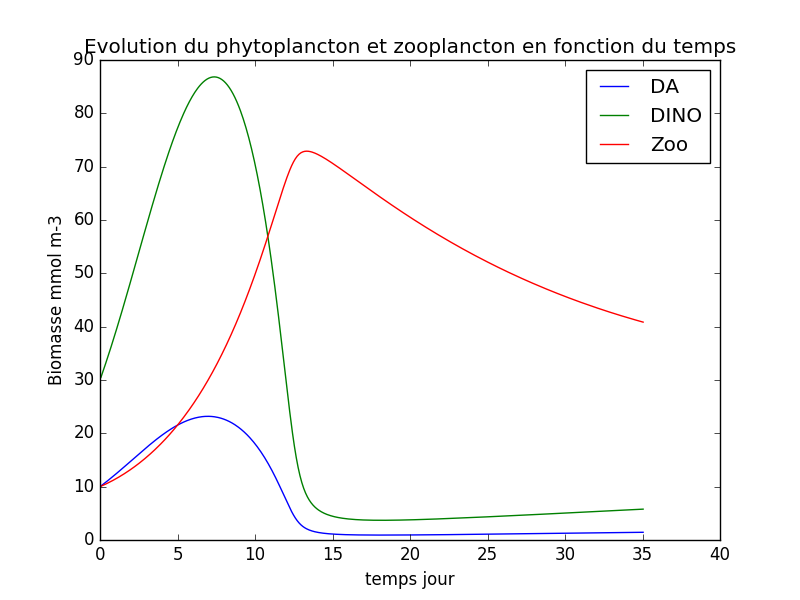
\includegraphics[width=.5\textwidth]{partie2/test2sel.png}\hfill
  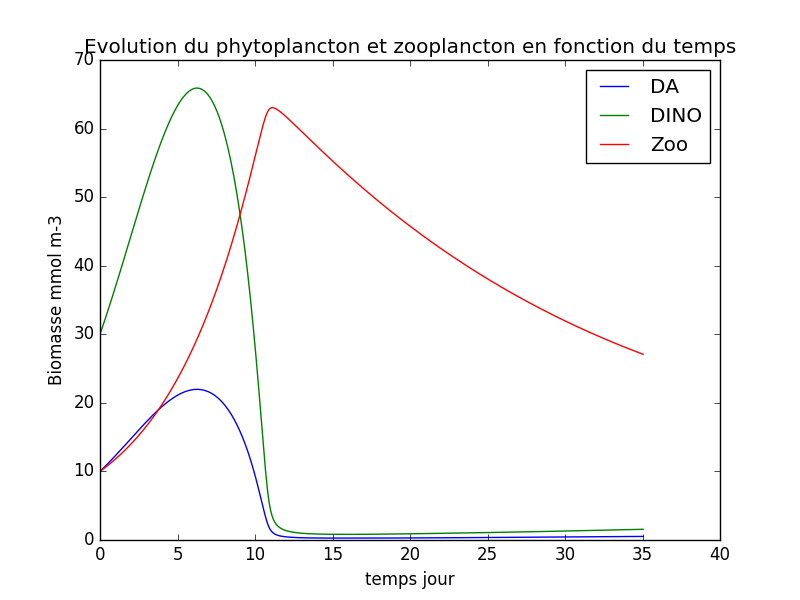
\includegraphics[width=.5\textwidth]{partie2/test2nonsel.png}
  \caption{\todo}
  \label{fig:partie2Test1}
\end{figure}
\begin{figure}
  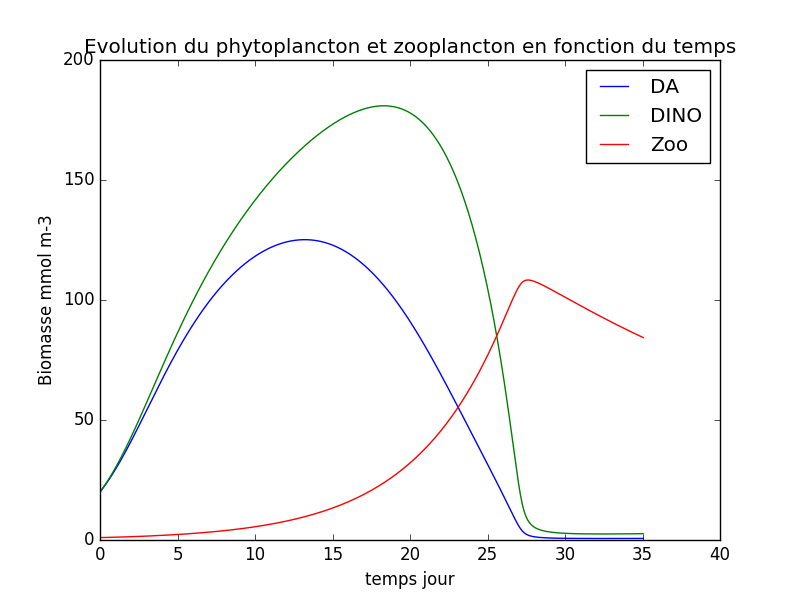
\includegraphics[width=.5\textwidth]{partie2/test3sel.png}\hfill
  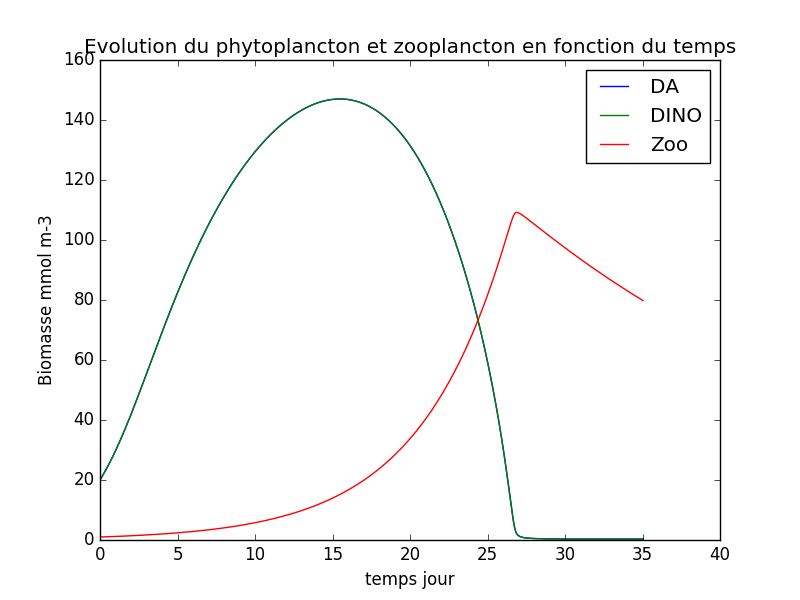
\includegraphics[width=.5\textwidth]{partie2/test3nonsel.png}\\
  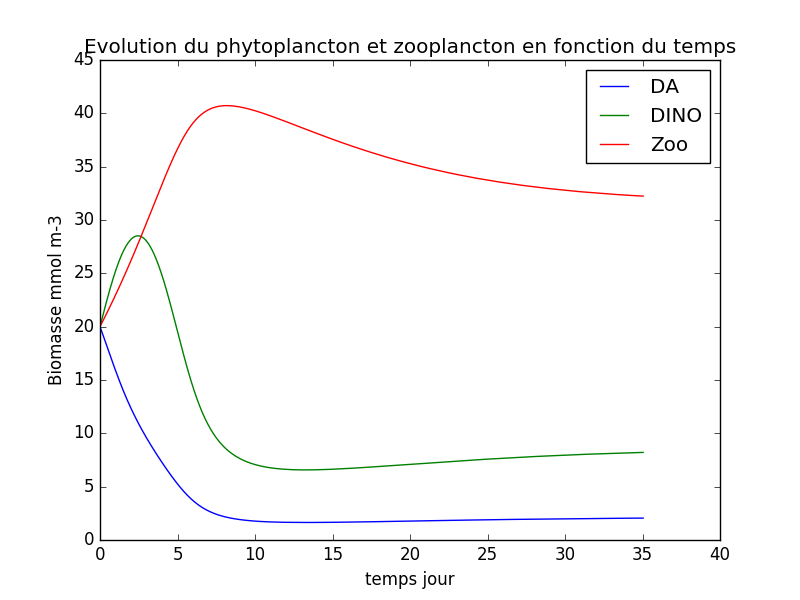
\includegraphics[width=.5\textwidth]{partie2/test4sel.png}\hfill
  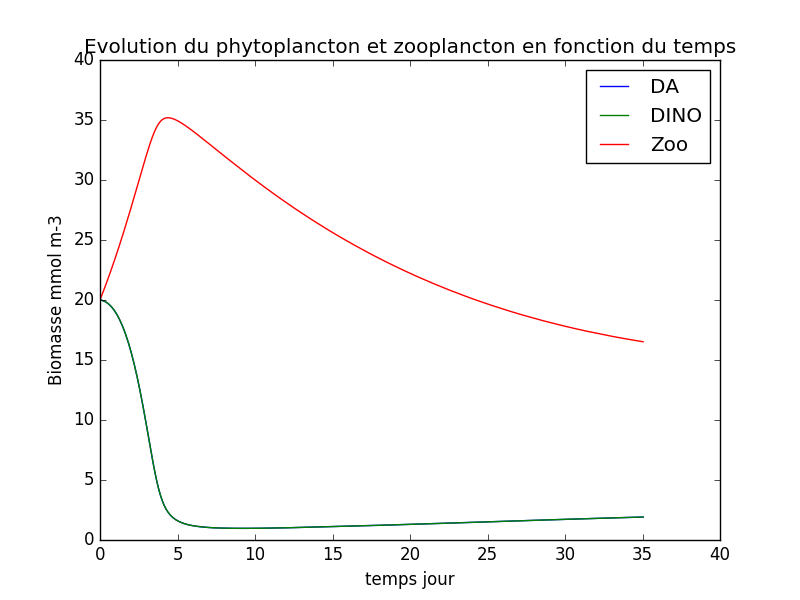
\includegraphics[width=.5\textwidth]{partie2/test4nonsel.png}
  \caption{\todo}
  \label{fig:partie2Test2}
\end{figure}


\subsection{Ref non selec}



\subsection{Ref selec}


\subsection{Test 1 non selec}

Ici, bien que les constantes de demi saturation des taux de grazing soient les mêmes, les concentrations initiales en Diatomées et Dinoflagellés sont différentes. Ainsi, puisque la concentration en Diatomées est diminuée de 10 mais que la concentration en Dinoflagellés est augmentée de 10, et que les deux populations de phytoplancton ont exactement les mêmes paramètres, l'évolution du zooplancton est exactement la même que dans le cas de la référence. Cependant, les Diatomées atteignent une concentration maximum beaucoup plus élevée que dans le cas de la référence (65 mmol.m-3), tandis que la concentration maximum des Dinoflagellés est plus faible (20 mmol.m-3). La somme des concentrations du phytoplancton est exactement la même que dans le cas de la référence, puisqu'une fois de plus, les deux populations de phytoplancton ont exactement les mêmes paramètres.

\subsection{Test 1 selec}

Dans cette simulation, l'affinité pour les Dinoflagellés est plus faible que pour les Diatomées. Cependant, la concentration initiale en Dinoflagellés est plus faible que dans le cas de la référence, ce qui explique que la concentration maximum en Dinoflagellés atteinte est plus faible que dans le cas de la référence.
De la même manière, l'affinité pour les Diatomées est plus grande, mais la concentration initiale en Diatomées est plus grande, ce qui explique que la concentration maximum en Diatomées est plus élevée que dans le cas de la référence.
De plus, puisque l'affinité pour les Diatomées est plus grande et que la concentration initiale en Diatomées est plus grande, le maximum de biomasse est atteint plus rapidement. 
La concentration maximum en zooplancton est cependant plus faible que dans le cas de la référence. Ainsi, augmenter la concentration initiale de la proie préférée entraîne une diminution du maximum du zooplancton. 

\subsection{Test 2 non selec}

La concentration initiale des Dinoflagellés a été augmentée de 10 mmol.m-3, tandis que la concentration initiale des Diatomées a été diminuée de 10 mmol.m-3. Ici aussi, tous les paramètres des deux populations de phytoplancton sont les mêmes. Ainsi, la concentration maximum en Dinoflagellés est plus importante que dans le cas de la référence, et la concentration maximum en Diatomées est plus faible. Cependant, la somme des deux concentrations des deux populations de phytoplancton est la même que dans le cas de la référence, et ainsi, l'évolution du zooplancton l'est aussi.

\subsection{Test 2 selec}

La concentration initiale en Dinoflagellés, qui sont moins appréciés que les Diatomées, est plus grande que dans le cas de la référence. Inversement, la concentration initiale des Diatomées est plus faible. Ainsi, cette situation mène à un taux de grazing des Diatomées faible, comme on peut le remarquer dans l'équation (REF EQ. TAUX GRAZING DA), et à un taux de grazing des Dinoflagellés élevé, comme on peut le remarquer dans l'équation (REF EQ. TAUX GRAZING DINO). Ceci permet aux Diatomées de croître sur une plus longue période, et d'atteindre un maximum de biomasse relativement plus grand que dans le cas de la référence. Inversement, la population de Dinoflagellés atteint un maximum relativement plus faible, et atteint ce maximum plus tôt que dans le cas de la référence. De plus, on peut voir que diminuer la concentration de la proie la plus appréciée entraîne une augmentation du maximum de concentration du zooplancton.

\subsection{Test 3 nonselec}

Ici, les concentrations initiales ainsi que tous les paramètres sont les mêmes pour les deux espèces de phytoplancton. Cependant, la concentration initiale en zooplancton est 10 fois plus faible que dans le cas de la référence. Ainsi, les deux espèces de phytoplancton croissent pendant une plus longue période, et atteignent donc un maximum de biomasse plus important. Puisque ces populations de phytoplancton atteignent un maximum de biomasse plus tard, alors le zooplancton atteint aussi le sien plus tard, et celui-ci est donc plus grand. 

\subsection{Test 3 selec}

Dans cette simulation, la concentration initiale en zooplancton est 10 fois inférieure que dans le cas de la référence. Ceci permet aux deux populations de phytoplancton de croître plus longtemps et donc d'atteindre des maxima de concentration plus grands. Ainsi, la population de zooplancton peut aussi croître plus longtemps et donc atteindre une concentration maximum plus grande. De plus, les Diatomées étant l'espèce la plus appréciée par le zooplancton, celle-ci atteindra son maximum avant les Dinoflagellés.

\subsection{Test 4 non selec}

Dans cette simulation, la concentration initiale en zooplancton est doublée par rapport à la référence. Ainsi, la pression de grazing est telle qu'elle empêche toute croissance des deux populations de phytoplancton. En effet, cette concentration initiale importante fait que le terme de mortalité des deux espèces phytoplanctoniques est toujours supérieur au terme de croissance (REF EQ. dDA/dt et dDINO/dt).

\subsection{Test 4 selec}

De la même manière que dans la simulation précédente, la concentration initiale du zooplancton est tellement grande qu'elle empêche la croissance des Diatomées, qui sont les proies préférées. En effet, le terme de croissance est toujours inférieur au terme de mortalité, dans l'équation de l'évolution des Diatomées. Cependant, la population de Dinoflagellés peut quand même croître, car le zooplancton a une affinité plus faible pour ceux-ci.

\subsection{Conclusion}

Nous pouvons constater que dans le cas d'un grazing non sélectif, si nous modifions les concentrations initiales des populations de phytoplancton, mais que la somme de ces concentrations restent les mêmes, alors l'évolution du zooplancton reste la même. Si nous gardons les mêmes conditions initiales pour les deux populations de phytoplancton, alors les deux populations vont suivre exactement la même évolution. Cela est du au fait que tous les paramètres, pour les deux populations de phytoplancton, sont les mêmes. En réalité, même si le grazing du zooplancton n'est pas sélectif, nous devrions observer des différences entre les évolutions des populations de phytoplancton.
De plus, nous pouvons constater que le zooplancton a toujours une concentration plus grande quand le grazing est sélectif que quand il est non sélectif. En effet, dans le cas sélectif, nous avons diminué l'affinité du zooplancton pour une des espèces, par rapport au cas non sélectif. Si nous avions augmenté l'affinité pour une des espèces, nous aurions observé une tendance totalement inverse.
